%% abtex2-modelo-trabalho-academico.tex, v-1.9.7 laurocesar
%% Copyright 2012-2018 by abnTeX2 group at http://www.abntex.net.br/ 
%%
% ------------------------------------------------------------------------
% ------------------------------------------------------------------------
% abnTeX2: Modelo de Trabalho Academico (tese de doutorado, dissertacao de
% mestrado e trabalhos monograficos em geral) em conformidade com 
% ABNT NBR 14724:2011: Informacao e documentacao - Trabalhos academicos -
% Apresentacao
% ------------------------------------------------------------------------
% ------------------------------------------------------------------------

\documentclass[
	% -- opções da classe memoir --
	12pt,				% tamanho da fonte
	openany,			% capítulos começam em pág ímpar (insere página vazia caso preciso)
	oneside,			% para impressão. Oposto a twoside
	a4paper,			% tamanho do papel. 
	% -- opções da classe abntex2 --
    % chapter=TITLE,		% títulos de capítulos convertidos em letras maiúsculas
	% section=TITLE,		% títulos de seções convertidos em letras maiúsculas
	% subsection=TITLE,	% títulos de subseções convertidos em letras maiúsculas
	% subsubsection=TITLE,% títulos de subsubseções convertidos em letras maiúsculas
    sumario=tradicional,
	% -- opções do pacote babel --
	english,			% idioma adicional para hifenização
	brazil				% o último idioma é o principal do documento
	]{abntex2}

% ---
% Pacotes básicos 
% ---
\usepackage{lmodern}			% Fonte Latin Modern		
% \usepackage{mathptmx}       	% Fonte Times New Roman Equivalente
\usepackage[T1]{fontenc}		% Selecao de codigos de fonte.
\usepackage[utf8]{inputenc}		% Codificacao do documento (conversão automática dos acentos)
\usepackage{indentfirst}		% Indenta o primeiro parágrafo de cada seção.
\usepackage{color}				% Controle das cores
\usepackage{graphicx}			% Inclusão de gráficos
\usepackage{microtype} 			% para melhorias de justificação
\usepackage{titlesec} 
\usepackage[portuguese]{nomencl}
\usepackage{siunitx}
\usepackage{amssymb}
\usepackage{csquotes}
\usepackage{etoolbox}
\usepackage{textcomp}
\usepackage{gensymb}
\usepackage{amsmath}
\usepackage{amssymb}
\usepackage{bbold}
\usepackage{soul}
% \usepackage[round]{natbib} % bibliografias
% \bibliographystyle{abnt}
\usepackage[
style = abnt, % Sistema alfabético
% style = abnt-numeric, % Sistema numérico
% style = abnt-ibid, % Notas de referência
giveninits,
indent,
justify,
uniquename=init,
]{biblatex}
\addbibresource{references.bib}

\usepackage{ragged2e} % justificação
\usepackage[linewidth=1pt]{mdframed} %Caixa com borda

% ---
% Informações de dados para CAPA e FOLHA DE ROSTO
% ---

\titulo{\MakeUppercase{Template de documento}}
\autor{Gustavo Pretto Scholze}
\local{Brasil}
\data{2023}
\orientador{Nome do Orientador}
\tipotrabalho{Tipo de trabalho}


\preambulo{Trabalho apresentado ao Departamento de Engenharia X da Escola de Engenharia da Universidade Federal do Rio Grande do Sul, como parte dos requisitos para obtenção do tanananan.}
% ---

\newcommand{\coordenador}{Coordenador do Curso} % COORDENADOR DO CURSO
\newcommand{\areaconcentracao}{Área de concentração}

\newcommand\imprimecomissao[1]{\hspace{3cm}Prof. #1 \\\vspace*{1\baselineskip} } % FORMATAÇÃO DA BANCA
\newcommand{\comissao}{Fulano A,Fulano B, Fulano C} %   LISTA DE PROFESSORES DA BANCA {A,B,C,D,...}


% ---
% informações do PDF
\makeatletter
\hypersetup{
     	% pagebackref=true,
		pdftitle={\@title}, 
		pdfauthor={\@author},
    	pdfsubject={\imprimirpreambulo},
	    pdfcreator={},
		pdfkeywords={SMP}{trabalho acadêmico}, 
		colorlinks=false,       		% false: boxed links; true: colored links
    	linkcolor=blue,          	% color of internal links
    	citecolor=blue,        		% color of links to bibliography
    	filecolor=magenta,      		% color of file links
		urlcolor=blue,
		bookmarksdepth=4,
        hidelinks,
}
\makeatother
\newcommand{\etal}{\textit{et al.}} % COMANDO ET AL.
\makeatletter

\setlength{\@fptop}{5pt} % Set distance from top of page to first float
\makeatother
% ---

% ---
% Possibilita criação de Quadros e Lista de quadros.
% Ver https://github.com/abntex/abntex2/issues/176
%
\newcommand{\quadroname}{Quadro}
\newcommand{\listofquadrosname}{Lista de quadros}

\newfloat[chapter]{quadro}{loq}{\quadroname}
\newlistof{listofquadros}{loq}{\listofquadrosname}
\newlistentry{quadro}{loq}{0}

% configurações para atender às regras da ABNT
\setfloatadjustment{quadro}{\centering}
\counterwithout{quadro}{chapter}
\renewcommand{\cftquadroname}{\quadroname\space} 
\renewcommand*{\cftquadroaftersnum}{\hfill--\hfill}

\setfloatlocations{quadro}{hbtp} % Ver https://github.com/abntex/abntex2/issues/176
% ---

% --- 
% Espaçamentos entre linhas e parágrafos 
% --- 

% O tamanho do parágrafo é dado por:
% \setlength{\parindent}{1.3cm}

% Controle do espaçamento entre um parágrafo e outro:
\renewcommand{\baselinestretch}{1}  %altura da linha 1.0
\parindent=1cm %TAMANHO DA IDENTAÇÃO
% ---
% compila o indice
% ---
\makeindex
% ---

% FONTE GRANDE TEM QUE SER SETADA MANUALMENTE PARA 14pt
\makeatletter
\renewcommand\large{\@setfontsize\large{14pt}{12}} %muda tamanho da fonte grande
\makeatother

\newcommand{\spacesize}{\the\fontdimen2\font} % LARGURA DE UM ESPAÇO

% FORMATA FONTES DE SEÇÕES, CAPÍTULOS ...
% Capitulo
\titleformat{\chapter}
  {\normalfont\bfseries \large}{\thechapter.}{\spacesize}{\MakeUppercase}
\titlespacing{\chapter}{0em}{12pt}{12pt}
% Seção
\titleformat{\section}
  {\normalfont\bfseries\normalsize}{\thesection.}{\spacesize}{}
\titlespacing{\section}{0em}{12pt}{12pt}
% Subseção
\titleformat{\subsection}
  {\normalfont\bfseries\normalsize}{\thesubsection.}{\spacesize}{}
\titlespacing{\subsection}{0em}{12pt}{12pt}
% Subsubseção
\titleformat{\subsubsection}
  {\normalfont\bfseries\normalsize}{\thesubsubsection.}{\spacesize}{}
\titlespacing{\subsubsection}{0em}{12pt}{12pt}

% \pagenumbering{roman}               %NUMERAÇÃO ROMANA
\makenomenclature % CRIA A NOMENCLATURA

%                       SUMARIO
% ---
% ---
% ---
\renewcommand{\tocheadstart}{\normalfont} %FONTE USADA
\renewcommand{\ABNTEXchapterfont}{\normalfont\bfseries} %FONDE DOS CAPITULOS
\renewcommand{\ABNTEXchapterfontsize}{\large} %TAM DA FONTE DOS CAPITULOS

\renewcommand\cftchapteraftersnumb{\normalfont\bfseries .\hspace{\spacesize}} %ADICIONA . DEPOIS DO NÚMERO DO CAPÍTULO
\renewcommand\cftsectionfont{\normalfont\uppercase} %MUDA FONTE DA SEÇÃO NO SUMARIO

\makeatletter
\settocpreprocessor{chapter}{% CAPITALIZA CAPITULOS (\UPPERCASE E \MAKEUPPERCASE NÃO FUNCIONAM COM O HYPEREF)
\let\tempf@rtoc\f@rtoc%
\def\f@rtoc{%
\texorpdfstring{\MakeTextUppercase{\tempf@rtoc}}{\tempf@rtoc}}%
}
\renewcommand\cftparskip{.2em} %ESPAÇAMENTO LINHAS DO SUMARIO
\renewcommand\cftdotsep{.8} %ESPAÇAMENTO ENTRE PONTOS DE SEOARAÇÃO 
\renewcommand\chapternumberlinebox[2]{#2} %TIRA ESPAÇAMENTO DO PONTO
% ---
% ---
% ---



\usepackage{pdfpages} %CARREGA PDF COMO PÁGINAS
\makeatother

\usepackage{float} %POSSIBILITA POSICIONAR FIGURAS E TABELAS  NO LOCAL INSERIDO COM [H]
\usepackage{tcolorbox} %PARA A FORMATAÇÃO DO RESUMO

\tcbuselibrary{breakable, skins}

% MACROS PARA INSERIR  OS TERMOS FIGURA E TABELA NO TEXTO 
\newcommand{\figura}{Figura}
\newcommand{\figuras}{Figuras}
\newcommand{\tabela}{Tabela}


% DEFINIÇÃO DA NOMENCLATURA
% %% CRIA GRUPOS DA NOMENCLATURA
% -----------------------------------------
\renewcommand\nomgroup[1]{%
  \item[\bfseries
  \ifstrequal{#1}{S}{\textnormal{Símbolos}}{
  \ifstrequal{#1}{A}{\textnormal{Abreviaturas e acrônimos}}{
  Outros Símbolos
  }}%
]}
% -----------------------------------------
%% POSSIBILITA UNIDADES NA NOMENCLATURA
%----------------------------------------------
\newcommand{\nomunit}[1]{%
\renewcommand{\nomentryend}{\hspace*{\fill}#1}}
%----------------------------------------------

% ABREVIAÇÕES E SIGLAS

\nomenclature[A]{SMP}{Polímeros com memória de forma}
\nomenclature[A]{KKT}{Karush Kuhn Tucker}
\nomenclature[A]{SME}{Efeito de memória de forma}
\nomenclature[A]{TCP}{Protocolo de Controle de Transmissão}
\nomenclature[A]{IP}{Protocolo de Internet}
% COMANDOS PARA INSERIR UNIDADES 
\newcommand{\MPa}{\nomunit{\SI{}{\mega \pascal}}}
\newcommand{\K}{\nomunit{\SI{}{\kelvin}}}

% SÍMBOLOS

\nomenclature[S]{$E_g$}{Módulo de elasticidade na fase vítrea \nomunit{\SI{}{\mega \pascal}}}
\nomenclature[S]{$E_r$}{Módulo de elasticidade na fase emborrachada \nomunit{\SI{}{\mega \pascal}}}
\nomenclature[S]{$\nu_g$}{Coeficiente de Poisson na fase vítrea}
\nomenclature[S]{$\nu_r$}{Coeficiente de Poisson na fase emborrachada}
\nomenclature[S]{$c$}{Coeficiente de afixamento imperfeito}
\nomenclature[S]{$c^p$}{Coeficiente de retorno imperfeito}
\nomenclature[S]{$Z_g$}{Fração volumétrica entre fases}
\nomenclature[S]{$\mathbb{1}$}{Tensor Unitário}
\nomenclature[S]{$R_{pg}$}{Limite de Escoamento \MPa}



\nomenclature[S]{$\lambda$}{Primeiro parâmetro de Lamé}
\nomenclature[S]{$\mu$}{Segundo parâmetro de Lamé}
\nomenclature[S]{$\theta_{glassy}$}{Temperatura vítrea \K}
\nomenclature[S]{$\theta_{rubbery}$}{Temperatura emborrachada \K}

\nomenclature[S]{$\theta_{cool}$}{Temperatura de Transição no arrefecimento \K}
\nomenclature[S]{$\theta_{heat}$}{Temperatura de Transição no aquecimento \K}
\nomenclature[S]{$\omega_{heat}$}{Suavidade da curva no aquecimento \nomunit{\SI{}{\kelvin^{-1}}}}
\nomenclature[S]{$\omega_{cool}$}{Suavidade da curva no arrefecimento \nomunit{\SI{}{\kelvin^{-1}}}}
\nomenclature[S]{$\omega_{trans}$}{Suavidade da da solidificação \nomunit{\SI{}{\kelvin^{-1}}}}

\nomenclature[S]{$\sigma_r$}{Tensor tensão de Cauchy da fase emborrachada \nomunit{\SI{}{\mega \pascal}}}
\nomenclature[S]{$\sigma_g$}{Tensor tensão de Cauchy da fase vítrea \nomunit{\SI{}{\mega \pascal}}}
\nomenclature[S]{$\sigma$}{Tensor tensão de Cauchy total \nomunit{\SI{}{\mega \pascal}}}

\nomenclature[S]{$\mathbf{S}_r$}{Segundo tensor de Piola-Kirchhoff da fase emborrachada \MPa}
\nomenclature[S]{$\mathbf{S}_g$}{Segundo tensor de Piola-Kirchhoff da fase vítrea \MPa}
\nomenclature[S]{$\mathbf{X}_g$}{Tensão termodinâmica plástica \MPa}

\nomenclature[S]{$\mathbf{C}$}{Tensor direito de deformação de Cauchy-Green}
\nomenclature[S]{$\mathbf{E}$}{Tensor de Green-Lagrange}

\nomenclature[S]{$\psi$}{Energia livre de Helmholtz \nomunit{\SI{}{\joule}}}
\nomenclature[S]{$\eta$}{Entropia \nomunit{\SI{}{\joule \cdot\kelvin^{-1}}}}
\nomenclature[S]{$U$}{Energia interna \nomunit{\SI{}{\joule}}}
\nomenclature[S]{$\dot{\gamma}$}{Incrementador de deformação plástica}
\nomenclature[S]{$\kappa$}{Condutividade térmica \nomunit{\SI{}{\watt \cdot\meter^{-1} \cdot \kelvin^{-1}}}}


\usepackage{lipsum} % PARA GERAR DUMMY TEXT NO TEMPLATE -> PODE SER REMOVIDO NO TRABALHO FINAL
% ----
% Início do documento
% ----
\begin{document}

\renewcommand{\imprimircapa}{%
\begin{capa}%
% \center
% {\ABNTEXchapterfont\large\imprimirautor}
% \vspace*{\fill}
% {\ABNTEXchapterfont\bfseries\LARGE\imprimirtitulo}
% \vspace*{\fill}
% {\large\imprimirlocal}
% \par
% {\large\imprimirdata}
% \vspace*{1cm}
\center
  UNIVERSIDADE FEDERAL DO RIO GRANDE DO SUL
  \par
ESCOLA DE ENGENHARIA
  \par
  PROGRAMA DE PÓS-GRADUAÇÃO EM ENGENHARIA DE MINAS, METALÚRGICA E DE MATERIAIS 
\\~\\~\\~\\~\\
\imprimirtitulo
\\~\\
por\\~\\~\\
\imprimirautor
\\~\\~\\~\\~\\~\\
\begin{FlushRight}
\parbox{0.5\linewidth}{
\justifying
\parindent=0pt
Trabalho apresentado ao Departamento de \linebreak
Engenharia de Minas da Escola de \linebreak
Engenharia da Universidade Federal do Rio
Grande do Sul, como parte dos requisitos
para aprovação na disciplina de DISCIPLINA.}
\end{FlushRight}
\vspace*{\fill}
LOCAL, MÊS de ANO

\end{capa}}


\imprimircapa
\pretextual{}
% \includepdf[pages=-]{Document/Chapters/Preambulo/doc.pdf} %FOLHA DE ROSTO ->https://sabi.ufrgs.br/servicos/publicoBC/ficha.php

% \centering
\imprimirautor
\vspace*{5\baselineskip} %5 linhas em branco

\imprimirtitulo

\vspace*{3\baselineskip} %3 linhas em branco
\begin{mdframed}[leftmargin=1cm,rightmargin=0pt]
\centering
ESTA MONOGRAFIA FOI JULGADA ADEQUADA COMO PARTE DOS REQUISITOS PARA A OBTENÇÃO DO TÍTULO DE\\
\textbf{ENGENHEIRO MECÂNICO}\\
APROVADA EM SUA FORMA FINAL PELA BANCA EXAMINADORA DO
CURSO DE ENGENHARIA MECÂNICA
\vspace*{1\baselineskip} % linhas em branco

\raggedright
\parindent=0pt
\hspace{12em}Prof. \coordenador\\
\hspace{12em}Coordenador do Curso de Engenharia Mecânica
\end{mdframed}
\raggedright
\vspace*{1\baselineskip} % linhas em branco
Área de Concentração: \areaconcentracao\\
\vspace*{1\baselineskip} % linhas em branco
Orientador: \imprimirorientador\\
\vspace*{1\baselineskip} % linhas em branco
Comissão de Avaliação:\\
\vspace*{1\baselineskip} % linhas em branco
% \expandafter\forcsvlist\imprimecomissao\expandafter{\comissao}
\expandafter\forcsvlist\expandafter\imprimecomissao\expandafter{\comissao}  % folha de aprovação
% \vspace*{\fill}
AGRADECIMENTOS\\
\vspace*{\baselineskip} %linha em branco
\justifying


\lipsum[1]\\

\newpage
\vspace*{\fill}
EPÍGRAFE\\
\vspace*{\baselineskip} %linha em branco
\begin{FlushRight}


\textit{"\lipsum[1]"}\\


\vspace*{2\baselineskip} %linha em branco

\textit{Nome do autor da frase}
\end{FlushRight}

 % agradecimentos, epígrafe ...
\newpage
\large
\begin{center}
\large
UNIVERSIDADE FEDERAL DO RIO GRANDE DO SUL \linebreak
ESCOLA DE ENGENHARIA\linebreak
PROGRAMA DE PÓS-GRADUAÇÃO EM ENGENHARIA DE MINAS, METALÚRGICA E DE MATERIAIS
\end{center}
% \RaggedLeft
\raggedright
\vspace*{\baselineskip} %linha em branco
\textbf{\imprimirtitulo}
\vspace*{2\baselineskip} %linha em branco
\newtcolorbox{lmarginbox}{
  blanker, breakable, left=.5em,top=3pt,bottom=3pt,
  borderline west={3pt}{0pt}{black}} %MARGEM LATERAL

\newcommand{\email}{scholzegustavo@gmail.com}
\begin{lmarginbox}
\normalsize
\textbf{\imprimirautor}\\
\href{mailto:\email}{\email}

\vspace*{\baselineskip} %linha em branco
\textbf{\textit{Resumo.}} <\lipsum[1]> 

\vspace*{\baselineskip} %linha em branco
\textbf{\textit{Palavras-Chave:}}
<Tag 1, Tag 2, Tag 3, Tag 4>

\vspace*{\baselineskip} %linha em branco
\textbf{\textit{Abstract.}} \textit{<\lipsum[1]>}

\vspace*{\baselineskip} %linha em branco
\textbf{\textit{Keywords:}} <Tag 1, Tag 2, Tag 3, Tag 4>

\end{lmarginbox} %resumo e abstract

% IMPRIME A NOMENCLATURA
\printnomenclature
\newpage
\pdfbookmark[0]{\contentsname}{toc}

\renewcommand\contentsname{} % APAGA NOME DO SUMÁRIO ABNT PARA INSERIR MANUALMENTE NO ESTILO DO TEMPLATE V4
\chapter*{SUMÁRIO}
\begingroup
\let\clearpage\relax
\vspace{-3em} % the removed space. Set as appropriate
\tableofcontents*
\endgroup


\cleardoublepage

\textual{}
\parindent=1em
\justifying
\chapter{INTRODUÇÃO}

\lipsum[1-3]
{% \let\clearpage\relax  % REMOVE QUEBRA DE PÁGINA ENTRE CAPÍTULOS

\chapter{FUNDAMENTAÇÃO TEÓRICA}

\section{Equações}
\subsection{Tensor Cauchy-Green à direita}
\begin{equation}
    \mathbf{C}=\mathbf{F}^T \mathbf{F}
    \label{eq:cauchyGreen}
\end{equation}
Onde $\mathbf{F}$ é o gradiente de deformação.
Eq. \eqref{eq:cauchyGreen}

\section{Elementos Gráficos}
\subsection{Tabelas}
\begin{table}[H]
    \caption{Descrição da tabela}
    \centering
    \begin{tabular}{c|c}
        A  & B \\
        C & D
    \end{tabular}
    \label{tab:my_label}
\end{table}

\tabela \ref{tab:my_label}

\subsection{Imagens}
\begin{figure}[H]
    \centering
    \caption{Descrição da imagem}
    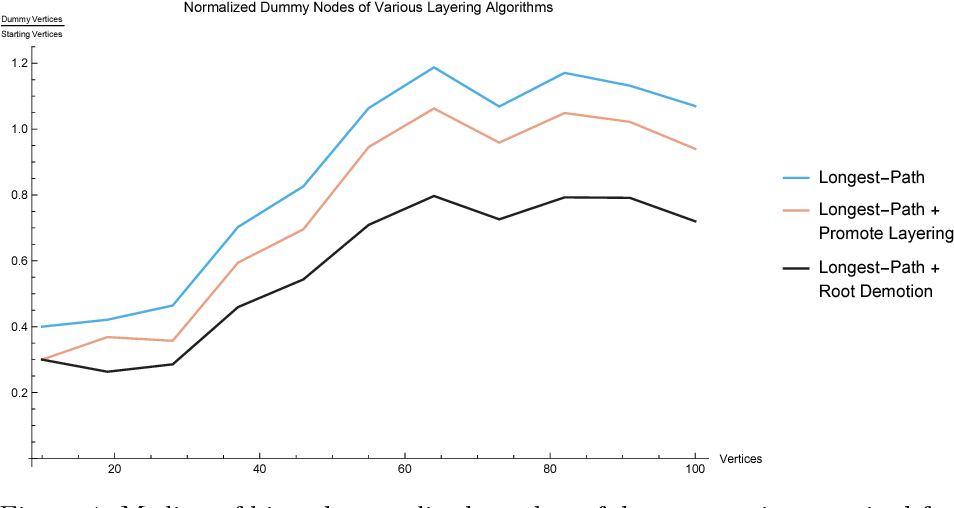
\includegraphics[width=.5\linewidth]{assets/fig.png}
    \label{fig:my_img}
\end{figure}

\section{Citações}
% \cite{Boatti2016AData}
\textcite{Boatti2016AData}
\textcite{Abrahamson2003ShapeResin}

\cite{Abrahamson2003ShapeResin}

\cites{Steven2014ShapeMateriability}{Haupt2002ContinuumMaterials}{Evangelista2010AStrain}

% \section{Otimização dos Parâmetros}
% \subsection{COBYLA}
% \subsection{Distância absoluta média}
% \subsection{Protocolo TCP/IP}



\chapter{METODOLOGIA}
\section{Seção}
\lipsum[1]
\subsection{Subseção}
\lipsum[1-10]




\chapter{RESULTADOS}
\label{resultados}

\lipsum[1-3]


\input{Document/Chapters/Conclusão}

\printbibliography

% \chapter*{APÊNDICE}
\addcontentsline{toc}{chapter}{APÊNDICE}
% \partapendices
\apendices
\chapter{Pseudocódigos}
\label{pseudocodigo}

\lipsum[5] % IMPRIME APENDICE

}
% \expandafter\string \normalsize\\
% \the\fontdimen2\font
\end{document}